% Name: Graph coloring
% Description: The Petersen graph colored with three colors, so no edge joins two vertices of the same color.
% Tags: graph coloring, Petersen graph, chromatic number

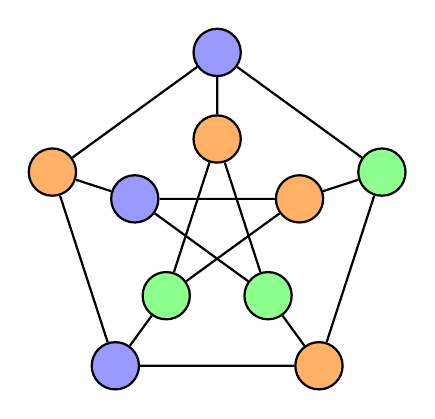
\begin{tikzpicture}[
  vertex/.style={circle, draw, thick, minimum size=6mm, inner sep=0pt},
  c1/.style={vertex, fill=blue!40},
  c2/.style={vertex, fill=orange!60},
  c3/.style={vertex, fill=green!45},
]
  \foreach \i/\c in {0/c1, 1/c2, 2/c1, 3/c2, 4/c3}
    \node[\c] (o\i) at ({90 + 72*\i}:2.2) {};
  \foreach \i/\c in {0/c2, 1/c1, 2/c3, 3/c3, 4/c2}
    \node[\c] (i\i) at ({90 + 72*\i}:1.1) {};
  \foreach \i in {0,...,4} {
    \pgfmathtruncatemacro\next{mod(\i + 1, 5)}
    \pgfmathtruncatemacro\skip{mod(\i + 2, 5)}
    \draw[thick] (o\i) -- (o\next) (o\i) -- (i\i) (i\i) -- (i\skip);
  }
\end{tikzpicture}
